\documentclass[a4paper,12pt]{article}
\usepackage{graphicx}
\graphicspath{ {imagesTex/} }
\usepackage{listings}


\begin{document}

El conjunto de nuestros datos cuenta con datos de $1917$ sujetos diferentes, de los cuales vamos a filtrar aquellas posiciones con informaci\'on relevante, es decir, cuya latitud y longitud no sea nula (es nula porque no se recibe bien la posici\'on). Para ello, ejecutamos la siguiente consulta con el fin de quedarnos con los 5 recursos con datos m\'as representativos. 

\begin{lstlisting}
mysql> select recurso, count(id) 
	   from posicionesgps 
	   where latitud <> 0 and longitud <> 0 
	   group by recurso order by 2 desc limit 5;
	   
	   +----------------+-----------+
	   | recurso        | count(id) |
	   +----------------+-----------+
	   | tetra:12082781 |     39839 |
	   | tetra:12082364 |     35858 |
	   | tetra:12086044 |     27532 |
	   | tetra:12082579 |     17574 |
	   | tetra:12082434 |     15257 |
	   +----------------+-----------+

\end{lstlisting}


\section{K-Means}

Vamos a realizar un clustering de K-medias utilizando Weka sobre el primer sujeto tetra:12082781, importamos la latitud, longitud y fecha en Weka con la siguiente consulta

\begin{lstlisting}
select latitud, longitud, UNIX_TIMESTAMP(fecha) from posicionesgps 
where latitud <> 0 and longitud <> 0 and recurso="tetra:12082781";
\end{lstlisting}

Si visualizamos los datos de latitud y longitud, obtenemos

Resultados: 

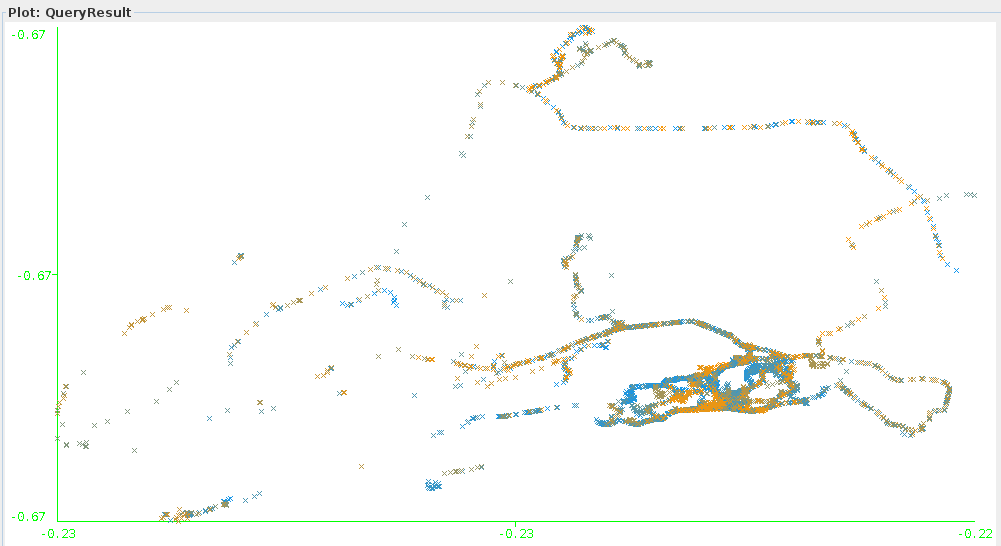
\includegraphics[scale=.5]{tetra:12082781.png}

\section{DJ-clustering}




\end{document}